\documentclass[11pt]{article}
\usepackage[a4paper,margin=25mm]{geometry}
\usepackage[T1]{fontenc}
\usepackage{lmodern}
\usepackage{microtype}
\usepackage{amsmath,amssymb,amsthm,mathtools}
\usepackage{booktabs,array,tabularx,longtable}
\usepackage{graphicx}
\usepackage{xcolor}
\usepackage{enumitem}
\usepackage{url}
\usepackage{caption}
\usepackage{float}
\usepackage[backend=biber,style=authoryear,maxcitenames=2,doi=true,url=true,isbn=false]{biblatex}
\addbibresource{references.bib}
\usepackage{hyperref}
\usepackage{cleveref}

\definecolor{deepteal}{HTML}{168C8C}
\definecolor{raspberry}{HTML}{B23A6F}
\definecolor{violet}{HTML}{6750A4}
\hypersetup{colorlinks=true,linkcolor=deepteal,citecolor=violet,urlcolor=raspberry,
 pdftitle={Conditional Sharp Partial Identification of Diversification Histories},
 pdfauthor={Anonymous agentic research candidate},
 pdfsubject={Birth-death congruence classes, partial identification, affine measure geometry},
 pdfkeywords={birth-death process, diversification, congruence class, partial identification, pulled speciation rate, deterministic survival event, sharp bounds}}

\newtheorem{theorem}{Theorem}
\newtheorem{proposition}[theorem]{Proposition}
\newtheorem{corollary}[theorem]{Corollary}
\newtheorem{lemma}[theorem]{Lemma}
\theoremstyle{definition}
\newtheorem{definition}[theorem]{Definition}
\newtheorem{remark}[theorem]{Remark}

\newcommand{\M}{\mathcal{M}}
\newcommand{\V}{\mathcal{V}}
\newcommand{\Fset}{\mathcal{F}}
\newcommand{\dd}{\,\mathrm{d}}
\newcommand{\ac}{\mathrm{ac}}

\title{\textbf{Conditional Sharp Partial Identification of Diversification Histories}\\
\large Affine Measure Geometry, Event Congruence and Certified Extremes}
\author{Anonymous agentic research candidate}
\date{Candidate release 0.2.1 --- 8 August 2026}

\begin{document}
\maketitle

\begin{abstract}
Extant timetrees identify a pulled diversification signal but do not generally identify time-varying speciation and extinction rates separately. Existing methods therefore construct or sample alternative histories in a congruence class. A finite cloud cannot certify a sharp endpoint, and its failure near an endpoint can be factorial in the discretisation dimension. Conditional on a fixed pulled speciation rate, we represent homogeneous birth--death histories by a cumulative-loss measure beneath an explicit survival barrier. Reciprocal speciation is affine in this measure and its Radon--Nikodym derivative with respect to pulled scale is the turnover ratio $\mu/\lambda$. We prove that the descendant-count law remains zero-inflated geometric under finitely many independent deterministic survival events and derive the complete fixed-stem reconstructed-tree density under stem-survival and fixed-tip-count conditioning. For continuous histories with $0\leq\mu/\lambda\leq c$, we obtain sharp pointwise bounds for every finite $c$. The common restriction $c\leq1$ excludes continuous negative net diversification; extending beyond it reveals a phase transition: for $c>1$, the speciation supremum becomes infinite past a calculable pulled scale. Finite external interval constraints yield explicit least and greatest trajectories, pairwise infeasibility witnesses, a positive-survival test and the minimum compatible turnover cap. We also derive an exact endpoint-sampling law showing why finite random exploration is not certification. A public mammal curve provides a plug-in sensitivity illustration only: no simultaneous pulled-signal band or fossil observation model is claimed. The contribution is exact conditional projection and certification, not a replacement for birth--death likelihoods, identifiable restricted models or fossilised birth--death inference.
\end{abstract}

\paragraph{Assurance boundary.}
This is an unrefereed theorem-led candidate. Internal replay, independent linear-programming checks, direct branching-process simulation and deliberate negative controls pass. External specialist review of the fixed-stem event theorem, a systematic priority search, simultaneous uncertainty for the pulled signal, a fossil observation bridge and an actual matched CRABS run remain open gates. ``Sharp'' always means sharp over the stated conditional model class.

\paragraph{Persistent identifier.}
Specific-version DOI: \href{https://doi.org/10.5281/zenodo.21851319}{10.5281/zenodo.21851319}.

\section{Decision problem and contribution}
Let $\tau\in[0,T]$ denote age before an analysis origin, with $\tau=0$ at that origin and larger $\tau$ further in the past. A homogeneous time-varying birth--death history has speciation rate $\lambda(\tau)>0$, extinction rate $\mu(\tau)\geq0$, and sampling probability $\rho\in(0,1]$ at the analysis origin. If $E(\tau)$ is the probability that a lineage at age $\tau$ leaves no sampled descendant, define
\begin{equation}
 u(\tau)=1-E(\tau),\qquad \lambda_p(\tau)=\lambda(\tau)u(\tau). \label{eq:definitions}
\end{equation}
The pulled speciation rate $\lambda_p$ is identified by the reconstructed extant-timetree likelihood under the generalized homogeneous model, whereas $\lambda$ and $\mu$ are not separately identified without further restrictions \parencite{louca2020,helmstetter2022}.

Existing tools construct or sample histories in the resulting congruence class \parencite{hohna2022,andreoletti2023,kopperud2023}. They answer an exploration question. The target here is a partial-identification question:
\begin{quote}
For a fixed pulled signal and explicit restrictions, what is the complete feasible trajectory set, what are the sharp extrema of a stated target, and which constraints explain infeasibility?
\end{quote}
The paper contributes four linked results. First, it identifies an affine positive-measure coordinate for the smooth fibre and a Stieltjes completion containing incomplete sampling and deterministic survival events. Second, it secures the finite-event result under a precisely stated fixed-stem conditioning convention. Third, it solves turnover-capped pointwise and finite-constraint identification, including the previously omitted $c>1$ regime. Fourth, it quantifies the failure of a transparent finite sampler to attain exact endpoints.

\section{Smooth affine fibre}
Assume that $\lambda_p$ is continuous and strictly positive and define
\begin{equation}
 F(\tau)=\exp\!\left\{\int_0^\tau\lambda_p(s)\dd s\right\},
 \qquad F(0)=1,\qquad F'=\lambda_pF. \label{eq:F}
\end{equation}
The survival probability satisfies
\begin{equation}
 u'=\lambda_p(1-u)-\mu u,\qquad u(0)=\rho. \label{eq:survival}
\end{equation}
Set
\begin{equation}
 A(\tau)=F(\tau)[1-u(\tau)]. \label{eq:A}
\end{equation}

\begin{theorem}[Smooth affine-fibre representation]\label{thm:smooth}
Fix $\lambda_p>0$ and $F$ from \eqref{eq:F}. The map
\[
 (\rho,\lambda,\mu)\longmapsto A=F\left(1-\frac{\lambda_p}{\lambda}\right)
\]
is a bijection between continuously differentiable histories with pulled rate $\lambda_p$ and functions $A\in C^1([0,T])$ satisfying
\[
 0\leq A(0)<1,\qquad A'\geq0,\qquad A<F.
\]
The inverse is
\begin{equation}
 \rho=1-A(0),\qquad u=\frac{F-A}{F},\qquad
 \lambda=\frac{\lambda_pF}{F-A},\qquad \mu=\frac{A'}{F-A}. \label{eq:inverse}
\end{equation}
If $\nu$ is the positive measure with cumulative function $A$, then
\begin{equation}
 \nu=(1-\rho)\delta_0+A'(\tau)\dd\tau,
 \qquad \frac{\dd\nu_{\ac}}{\dd F}=\frac{\mu}{\lambda}
 \quad\text{almost everywhere}. \label{eq:RN}
\end{equation}
\end{theorem}

\begin{proof}
Differentiate \eqref{eq:A}, use $F'=\lambda_pF$ and substitute \eqref{eq:survival}:
\[
 A'=\lambda_pF(1-u)-F\{\lambda_p(1-u)-\mu u\}=\mu uF\geq0.
\]
The initial value is $A(0)=1-\rho$, and $A<F$ is equivalent to $u>0$. Conversely, \eqref{eq:inverse} defines positive $u$ and $\lambda$ and non-negative $\mu$; direct substitution recovers \eqref{eq:survival} and $\lambda_p=\lambda u$. Finally,
\[
 \frac{\dd\nu_{\ac}}{\dd F}=\frac{A'}{F'}=\frac{\mu uF}{\lambda_pF}=\frac{\mu}{\lambda}.
\]
\end{proof}

At each age,
\begin{equation}
 \frac1{\lambda(\tau)}=\frac1{\lambda_p(\tau)}-
 \frac{A(\tau)}{\lambda_p(\tau)F(\tau)}, \label{eq:affine}
\end{equation}
so reciprocal speciation is affine in $\nu$. The admissible fibre
\begin{equation}
 \V_F=\{\nu\in\M_+([0,T]):\nu([0,\tau])<F(\tau)\ \forall\tau\} \label{eq:fibre}
\end{equation}
is convex and closed under pointwise meet and join of cumulative functions. It is not a cone because positive scaling can cross the barrier. Larger cumulative loss means larger $\lambda$, smaller $u$ and smaller $1/\lambda$.

\section{Measure completion and finite survival events}
For a finite positive Radon measure $\nu\in\V_F$, let
\begin{equation}
 A(\tau)=\nu([0,\tau]),\qquad q(\tau)=F(\tau)-A(\tau),\qquad u=q/F. \label{eq:q}
\end{equation}
Use right-continuous cumulative functions and let $q_-(\tau)=F(\tau)-A(\tau^-)$. Define
\begin{equation}
 \dd K(\tau)=\frac{\dd\nu(\tau)}{q_-(\tau)}. \label{eq:K}
\end{equation}

\begin{proposition}[Stieltjes loss equation]\label{prop:stieltjes}
The survival function solves
\begin{equation}
 \dd u=\lambda_p(1-u)\dd\tau-u_-\dd K. \label{eq:stieltjes}
\end{equation}
On the absolutely continuous part, $\dd K/\dd\tau=\mu$. If $\nu$ has an atom $m$ at age $a$, then
\begin{equation}
 u(a+)=s_au(a-),\qquad q(a+)=s_aq(a-),\qquad
 m=(1-s_a)q(a-), \label{eq:eventjump}
\end{equation}
where $s_a=1-m/q(a-)\in(0,1]$.
\end{proposition}

\begin{proof}
Since $u=1-A/F$ and $F$ is continuous,
\[
 \dd u=\lambda_p(1-u)\dd\tau-F^{-1}\dd A.
\]
Because $q_-=Fu_-$ and $\dd A=\dd\nu=q_-\dd K$, this is \eqref{eq:stieltjes}. The strict barrier gives $m<q(a-)$; taking jumps yields \eqref{eq:eventjump}.
\end{proof}

An atom at zero represents incomplete sampling. An interior atom represents independent deterministic survival of contemporaneous lineages. It is not a value of the continuous ratio $\mu/\lambda$.

\subsection{Descendant-count law}
Let $N_\tau$ be the number of sampled descendants at the analysis origin from one lineage at age $\tau$, with probability-generating function
\[
 G_\tau(z)=\mathbb E[z^{N_\tau}]=\sum_{k\geq0}p_k(\tau)z^k.
\]
Between events,
\begin{equation}
 \partial_\tau G=\lambda(G^2-G)+\mu(1-G),\qquad
 G_0(z)=1-\rho+\rho z. \label{eq:pgf}
\end{equation}
At an event with survival $s_a$, moving from the younger to the older side,
\begin{equation}
 G_{a+}(z)=1-s_a+s_aG_{a-}(z). \label{eq:pgfevent}
\end{equation}

\begin{theorem}[Zero-inflated geometric law with finite events]\label{thm:geometric}
For an absolutely continuous history with finitely many deterministic survival events,
\begin{equation}
 G_\tau(z)=1-u(\tau)+u(\tau)
 \frac{a(\tau)z}{1-[1-a(\tau)]z},
 \qquad a(\tau)=\frac1{F(\tau)}. \label{eq:zig}
\end{equation}
Thus
\begin{equation}
 p_0=1-u,\qquad p_k=\frac{u}{F}\left(1-\frac1F\right)^{k-1},\quad k\geq1, \label{eq:pk}
\end{equation}
and
\begin{equation}
 \frac{p_1}{u}=\frac1F,\qquad
 \Pr(N_\tau=k\mid N_\tau>0)=\frac1F\left(1-\frac1F\right)^{k-1}. \label{eq:conditionalgeometric}
\end{equation}
Finite events change $u$ but not the conditional positive descendant-count law.
\end{theorem}

\begin{proof}
At $\tau=0$, $a=1$ and \eqref{eq:zig} equals $1-\rho+\rho z$. Between events, $a'=-\lambda_pa=-\lambda ua$. Differentiate \eqref{eq:zig}, substitute $u'=\lambda u(1-u)-\mu u$ and $a'=-\lambda ua$, and recover \eqref{eq:pgf}. Uniqueness of the backward equation proves the form between events. Equation \eqref{eq:pgfevent} multiplies $u$ by $s_a$ without changing $a=1/F$, so the form persists across every event. Expanding the geometric series gives \eqref{eq:pk}--\eqref{eq:conditionalgeometric}.
\end{proof}

\subsection{Complete fixed-stem reconstructed-tree law}
Fix a stem age $T$. Let $0<t_1<\cdots<t_{n-1}<T$ be the ordered internal-node ages after marginalising over the exchangeable ranked topology. Conditional on the ages, the choice of splitting lineage and daughter orientation has a topology law that depends on $n$ and the reporting convention, but not on the rate history. Define
\begin{equation}
 h(t)=\lambda(t)p_1(t)=\frac{\lambda_p(t)}{F(t)}=-\frac{\dd}{\dd t}\frac1{F(t)}, \label{eq:h}
\end{equation}
so $\int_0^T h(t)\dd t=1-1/F(T)$.

\begin{theorem}[Finite-event congruence at fixed stem age]\label{thm:fixedstem}
Under \cref{thm:geometric}, the unconditioned joint density of $N_T=n$ and the ordered internal-node ages, with ranked topology marginalised, is
\begin{equation}
 g_{n,T}(t_1,\ldots,t_{n-1})=p_1(T)\prod_{i=1}^{n-1}i\lambda(t_i)p_1(t_i). \label{eq:unconditionedtree}
\end{equation}
It integrates to $p_n(T)$. Conditional on stem survival,
\begin{equation}
 f^{\mathrm{surv}}_{n,T}(t_1,\ldots,t_{n-1})
 =\frac{(n-1)!}{F(T)}\prod_{i=1}^{n-1}\frac{\lambda_p(t_i)}{F(t_i)}, \label{eq:survivaldensity}
\end{equation}
and conditional additionally on $N_T=n$,
\begin{equation}
 f^n_T(t_1,\ldots,t_{n-1})
 =\frac{(n-1)!}{[1-1/F(T)]^{n-1}}
 \prod_{i=1}^{n-1}\frac{\lambda_p(t_i)}{F(t_i)}. \label{eq:countdensity}
\end{equation}
Conditional on these ages, homogeneous branching and independent event thinning make the ranked-topology law exchangeable and independent of the rate history. Hence histories sharing $\lambda_p$ have the same complete fixed-stem reconstructed-tree law under either conditioning, including histories with finitely many independent deterministic survival events.
\end{theorem}

\begin{proof}
The branching property gives \eqref{eq:unconditionedtree} for the topology-marginal ordered ages. Before the first observed split the stem contributes $p_1(T)$. With $i$ reconstructed lineages, summing over which lineage generates the next observed split produces $i\lambda(t_i)$, and the new observed branch contributes $p_1(t_i)$. Conditional on that split, exchangeability makes the lineage choice uniform among the $i$ lineages; daughter orientation is likewise rate-independent. Independent event thinning preserves exchangeability and the recursion. By \eqref{eq:pk} and \eqref{eq:h},
\[
 g_{n,T}=\frac{u(T)}{F(T)}(n-1)!\prod_{i=1}^{n-1}h(t_i).
\]
Integration over the ordered simplex yields
\[
 \frac{u(T)}{F(T)}(n-1)!\frac1{(n-1)!}
 \left\{\int_0^Th(t)\dd t\right\}^{n-1}
 =\frac{u(T)}{F(T)}\left(1-\frac1{F(T)}\right)^{n-1}=p_n(T).
\]
Dividing by $u(T)$ proves \eqref{eq:survivaldensity}; dividing by the conditional geometric probability in \eqref{eq:conditionalgeometric} proves \eqref{eq:countdensity}.
\end{proof}

\begin{remark}[Conditioning scope]\label{rem:scope}
\Cref{thm:fixedstem} fixes stem age and covers stem-survival and observed-tip-count conditioning. It does not claim equality under random-origin priors, crown conditioning or other normalisers. Those cases require separate derivations. Event-aware reconstructed-process and coalescent point-process results remain the process-theoretic antecedents \parencite{lambert2013,hohna2015,macpherson2022}.
\end{remark}

\section{Turnover caps and the phase transition at \texorpdfstring{$c=1$}{c=1}}
In pulled-scale time $x=F(\tau)$, set $n(x)=A(F^{-1}(x))$ and $q(x)=x-n(x)$. For absolutely continuous histories,
\begin{equation}
 n'(x)=\frac{\mu}{\lambda}=: \varepsilon(x),\qquad
 q'(x)=1-\varepsilon(x),\qquad n(1)=1-\rho,\qquad q(1)=\rho. \label{eq:turnover}
\end{equation}
Assume no interior atoms and impose $0\leq\varepsilon\leq c$ for a finite $c\geq0$.

\begin{theorem}[Sharp pointwise bounds for every finite turnover cap]\label{thm:cap}
At any pulled scale $x\geq1$,
\begin{equation}
 q(x)\leq\rho+x-1, \label{eq:qupper}
\end{equation}
and
\begin{equation}
 \inf q(x)=\max\{\rho+(1-c)(x-1),0\}. \label{eq:qinf}
\end{equation}
The upper endpoint is attained by $\varepsilon=0$. The lower endpoint is attained by $\varepsilon=c$ when $\rho+(1-c)(x-1)>0$; otherwise zero is an unattained infimum because $q>0$. Consequently,
\begin{equation}
 \lambda_{\min}(x)=\frac{\lambda_p(x)x}{\rho+x-1}, \label{eq:lmin}
\end{equation}
while
\begin{equation}
 \sup\lambda(x)=
 \begin{cases}
 \displaystyle\frac{\lambda_p(x)x}{\rho+(1-c)(x-1)},&\rho+(1-c)(x-1)>0,\\[6pt]
 +\infty,&\rho+(1-c)(x-1)\leq0.
 \end{cases} \label{eq:lsup}
\end{equation}
\end{theorem}

\begin{proof}
Integrating $1-c\leq q'\leq1$ from $x=1$ gives the candidate endpoints while they remain positive. The upper endpoint follows from $\varepsilon=0$. If the lower affine expression is positive, $\varepsilon=c$ attains it. If it is non-positive, choose a constant $\varepsilon\leq c$ that gives any prescribed $q(x)=\delta>0$; along the linear path, $q$ remains positive. Letting $\delta\downarrow0$ proves the infimum. Since $\lambda=\lambda_px/q$, the rate bounds follow.
\end{proof}

\begin{corollary}[Three cap regimes]\label{cor:regimes}
The identification geometry has three regimes.
\begin{enumerate}[label=(\roman*)]
\item If $c<1$, the multiplicative width obeys
\begin{equation}
 \frac{\lambda_{\max}}{\lambda_{\min}}
 =\frac{\rho+x-1}{\rho+(1-c)(x-1)}\leq\frac1{1-c}. \label{eq:globalfactor}
\end{equation}
\item If $c=1$, both pointwise endpoints are finite and attained for every finite $x$, but the width $(\rho+x-1)/\rho$ has no uniform deep-time bound.
\item If $c>1$, define
\begin{equation}
 x_{\mathrm{crit}}=1+\frac{\rho}{c-1}. \label{eq:xcrit}
\end{equation}
The speciation supremum is finite below $x_{\mathrm{crit}}$ and infinite at and beyond it.
\end{enumerate}
\end{corollary}

The familiar assumption $c\leq1$ means $\mu\leq\lambda$ at every non-event time and therefore excludes continuous negative net diversification. The extension to $c>1$ makes the cost of allowing decline explicit rather than hiding it in a sampler.

\begin{figure}[t]
\centering
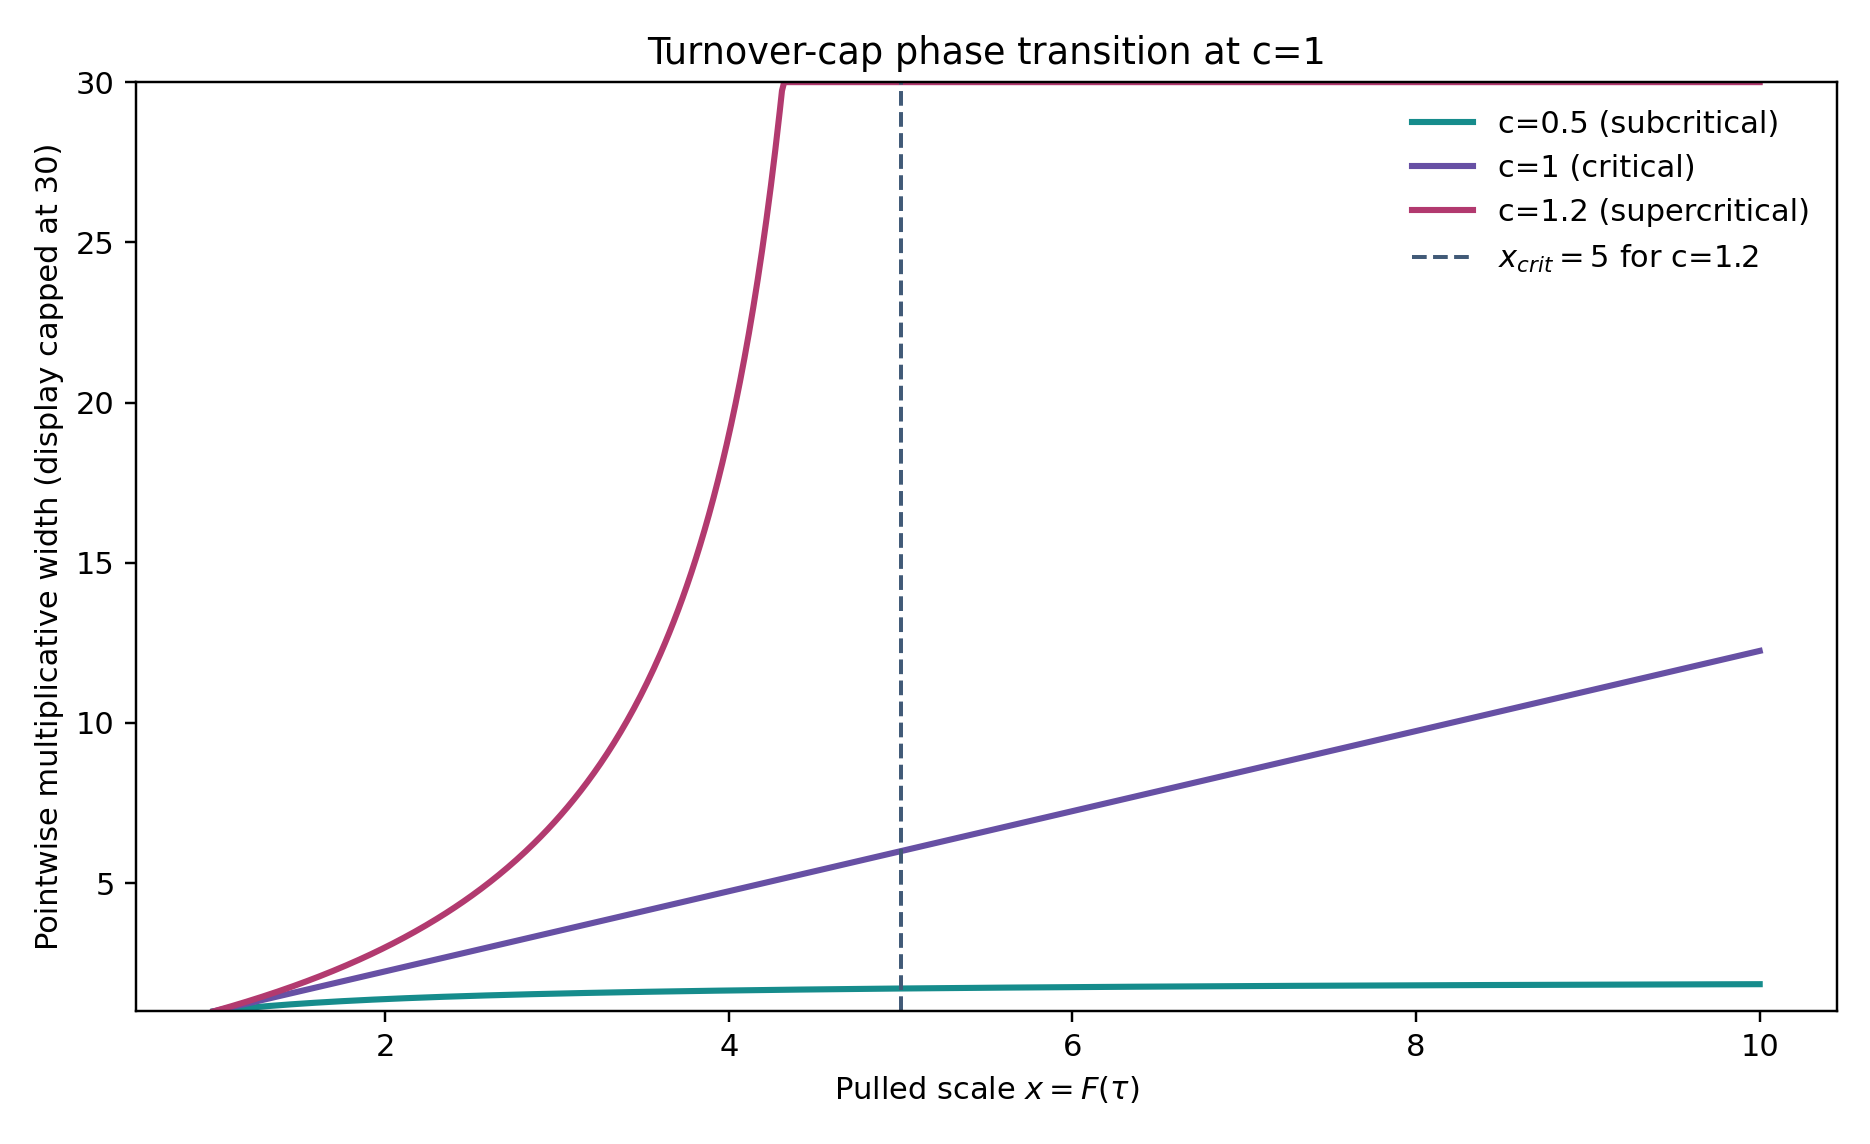
\includegraphics[width=0.88\linewidth]{figures/figure7_turnover_cap_phase.png}
\caption{Pointwise identification width for $\rho=0.8$. For $c<1$ the width has a finite global limit; at $c=1$ it grows without a global bound; for $c>1$ it diverges at the vertical critical pulled scale. The displayed width is capped at 30. These are conditional mathematical bounds, not empirical estimates.}
\label{fig:phase}
\end{figure}

\section{Finite constraints: exact envelopes and certificates}
Suppose external or structural information gives
\begin{equation}
 L_i\leq n(x_i)\leq U_i,\qquad 1\leq x_0<\cdots<x_m. \label{eq:intervals}
\end{equation}
The present anchor is normally included as $x_0=1$ and $L_0=U_0=1-\rho$.

\begin{theorem}[Directed-Lipschitz feasibility and sharp envelopes]\label{thm:envelopes}
There exists a non-decreasing, $c$-Lipschitz function satisfying \eqref{eq:intervals} if and only if
\begin{equation}
 L_i\leq U_j+c(x_i-x_j)_+\qquad\text{for every }i,j. \label{eq:pairwise}
\end{equation}
When feasible, the least and greatest such functions are
\begin{align}
 \underline n(x)&=\max_i\{L_i-c(x_i-x)_+\}, \label{eq:lowerenv}\\
 \overline n(x)&=\min_i\{U_i+c(x-x_i)_+\}. \label{eq:upperenv}
\end{align}
Every feasible $n$ obeys $\underline n\leq n\leq\overline n$, and both envelopes are feasible. A violating pair $(i,j)$ is a complete finite certificate of generic infeasibility.
\end{theorem}

\begin{proof}
Monotonicity and the slope cap imply
\[
 n(x)\geq L_i-c(x_i-x)_+,\qquad n(x)\leq U_i+c(x-x_i)_+.
\]
Taking the maximum and minimum gives the necessary bounds and \eqref{eq:pairwise}. Each lower cone is non-decreasing and $c$-Lipschitz, and pointwise maxima preserve both properties. Under \eqref{eq:pairwise}, $\underline n(x_j)\leq U_j$, while construction gives $\underline n(x_j)\geq L_j$; hence $\underline n$ is feasible and least. The upper proof is symmetric.
\end{proof}

\begin{corollary}[Positive-survival barrier]\label{cor:barrier}
Let the domain be $[1,X]$ and include the anchor $n(1)=1-\rho$. For $c\leq1$, generic feasibility in \cref{thm:envelopes} automatically implies $n(x)<x$. For $c>1$, a positive-survival history exists if and only if \eqref{eq:pairwise} holds and
\begin{equation}
 L_i<x_i\qquad\text{for every }i. \label{eq:barrierfinite}
\end{equation}
In that case the least envelope itself respects the barrier.
\end{corollary}

\begin{proof}
For $c\leq1$, the anchor and $n'\leq c$ give $n(x)\leq1-\rho+c(x-1)<x$. For $c>1$, consider one lower cone $\phi_i(x)=L_i-c(x_i-x)_+$. The function $\phi_i(x)-x$ increases up to $x_i$ and decreases afterwards, so its maximum is $L_i-x_i$. Hence, if every $L_i<x_i$, the least envelope $\underline n=\max_i\phi_i$ satisfies $\underline n(x)<x$ throughout the domain and supplies an admissible feasible history. Conversely, if $L_i\geq x_i$ for some $i$, every function satisfying that lower constraint has $n(x_i)\geq L_i\geq x_i$ and violates positive survival at $x_i$.
\end{proof}

\begin{corollary}[Minimum compatible turnover cap]\label{cor:mincap}
If $L_i\leq U_j$ whenever $x_i\leq x_j$, the smallest generic cap is
\begin{equation}
 c_\star=\max_{x_i>x_j}\frac{(L_i-U_j)_+}{x_i-x_j}. \label{eq:cstar}
\end{equation}
If some $x_i\leq x_j$ has $L_i>U_j$, monotonicity alone makes the system infeasible for every finite cap. A result $c_\star>1$ means that every absolutely continuous solution requires some negative-net-diversification interval, unless the data bridge, event structure or other assumptions change.
\end{corollary}

\begin{corollary}[Order-monotone targets]\label{cor:order}
Let $\Psi[n]$ be increasing under pointwise cumulative-loss order. Over a feasible set from \cref{thm:envelopes},
\[
 \inf\Psi=\Psi[\underline n],\qquad \sup\Psi=\Psi[\overline n],
\]
with reversed roles for decreasing targets. This covers point evaluations of $n$, $A$, $\lambda$ and the deterministic diversity quantity defined below, and positive weighted integrals of order-monotone transforms. Non-monotone targets, including peak timing and some path extrema, require a separate optimisation problem.
\end{corollary}

The two envelopes describe the pointwise projection of the functional identified set. An arbitrary curve drawn inside the shaded band need not satisfy the cross-time constraints.

\begin{figure}[t]
\centering
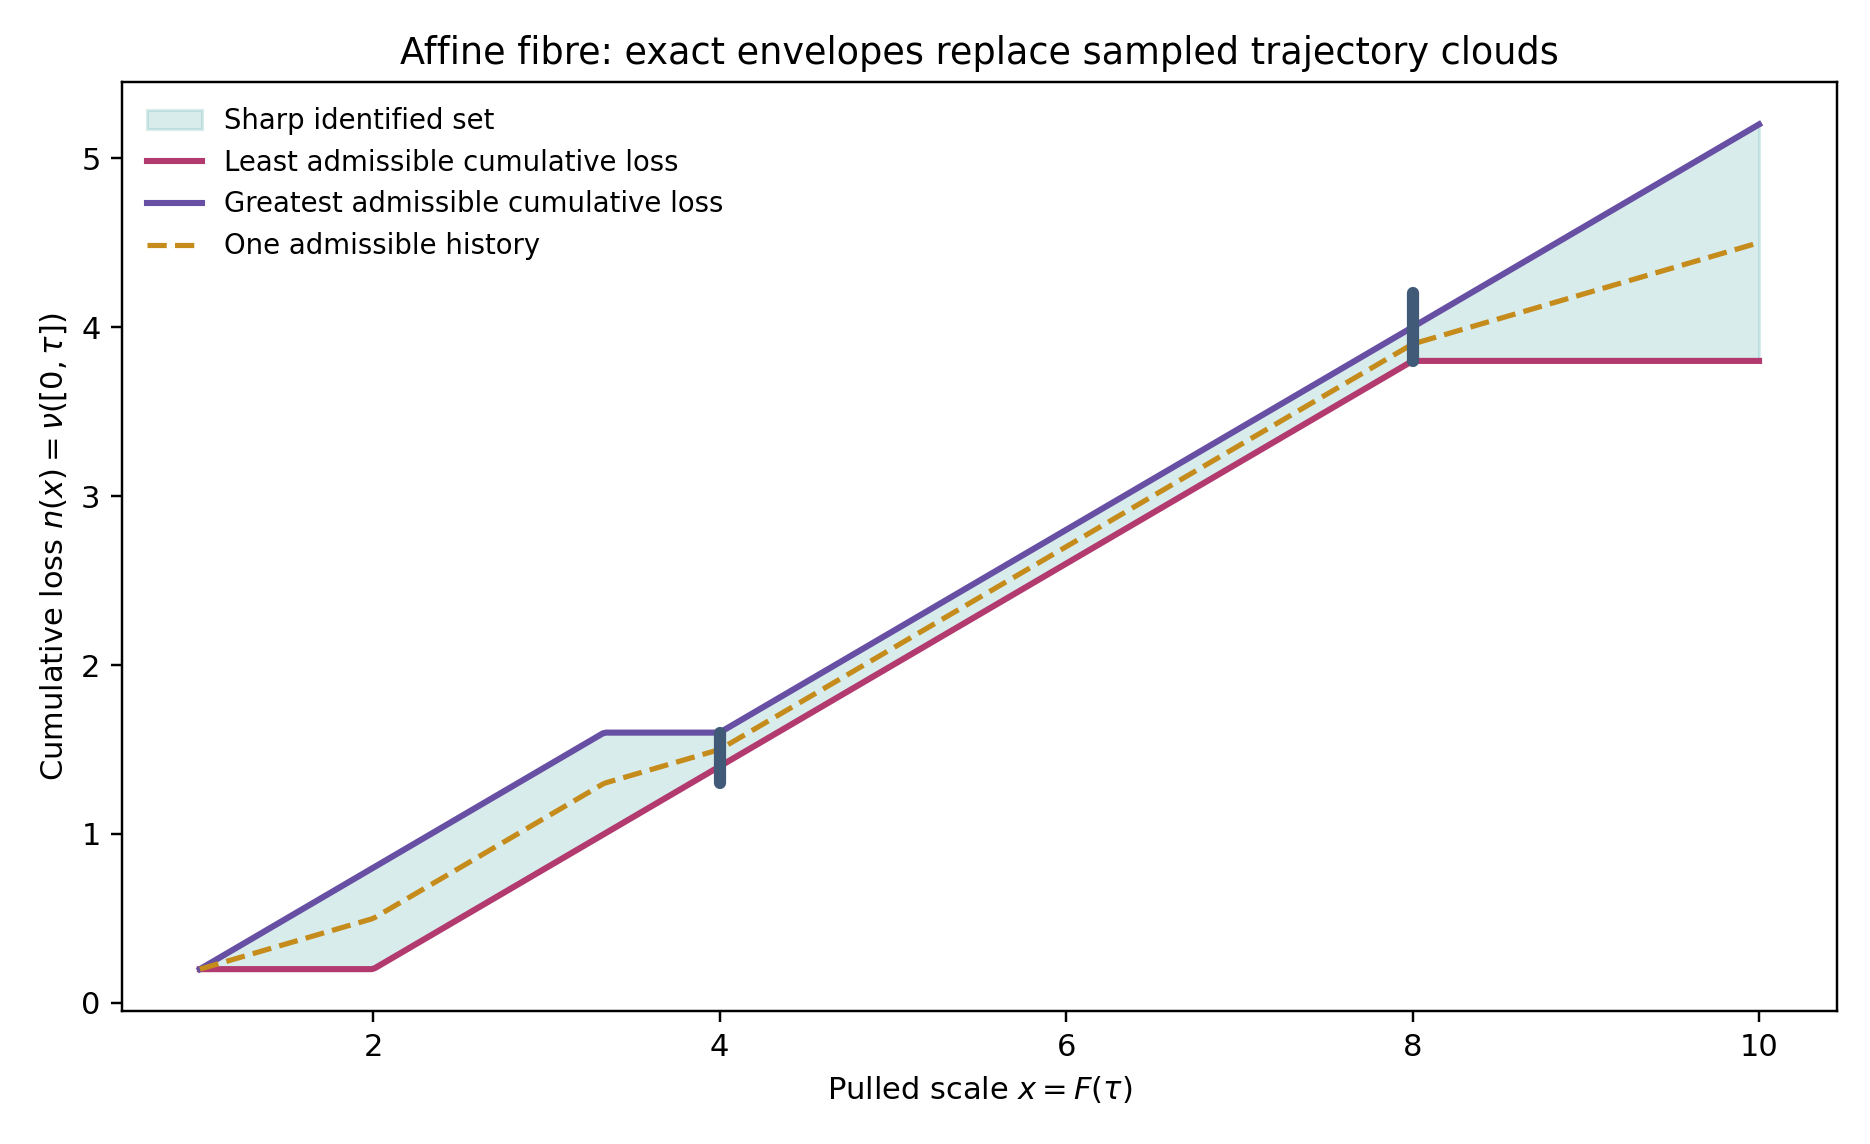
\includegraphics[width=0.88\linewidth]{figures/figure1_affine_geometry.png}
\caption{Least and greatest feasible cumulative-loss trajectories under finite interval constraints. The shading is the pointwise projection between two feasible extremal functions; it is not a licence to choose values independently at each $x$.}
\label{fig:geometry}
\end{figure}

\section{Why finite random sampling is not certification}
The distinction between exploration and certification can be quantified without criticising any particular implementation. Consider an equal pulled-scale grid $x_j=1+j\Delta$, $j=0,\ldots,m$, and independently draw each interval turnover $\varepsilon_j\sim\mathrm{Uniform}(0,c)$. The sharp maximal-loss endpoint is
\begin{equation}
 n_{\max}(x_m)=1-\rho+mc\Delta. \label{eq:nmax}
\end{equation}
A sampled endpoint has deficit
\begin{equation}
 D=n_{\max}(x_m)-n(x_m)=\Delta\sum_{j=1}^m(c-\varepsilon_j). \label{eq:deficit}
\end{equation}

\begin{theorem}[Factorial endpoint-sampling law]\label{thm:sampling}
Under the matched sampler above, $\Pr(D=0)=0$. For $0\leq\eta\leq c\Delta$,
\begin{equation}
 p_\eta:=\Pr(D\leq\eta)=\frac1{m!}\left(\frac{\eta}{c\Delta}\right)^m. \label{eq:smalltail}
\end{equation}
For $N$ independent sampled histories,
\begin{equation}
 \Pr\!\left(\min_{1\leq r\leq N}D_r\leq\eta\right)=1-(1-p_\eta)^N, \label{eq:bestofN}
\end{equation}
and the smallest $N$ giving probability at least $\gamma$ is
\begin{equation}
 N_{\min}=\left\lceil\frac{\log(1-\gamma)}{\log(1-p_\eta)}\right\rceil. \label{eq:Nmin}
\end{equation}
\end{theorem}

\begin{proof}
The variables $(c-\varepsilon_j)/c$ are independent $\mathrm{Uniform}(0,1)$. Exact endpoint attainment has probability zero. For $\eta/(c\Delta)\leq1$, the event that their sum is at most $\eta/(c\Delta)$ is an $m$-simplex of volume $[\eta/(c\Delta)]^m/m!$ inside the unit cube. Equations \eqref{eq:bestofN}--\eqref{eq:Nmin} follow from independent order statistics.
\end{proof}

With eight intervals and relative tolerance $\eta/(c\Delta)=0.2$, a 95\% hit probability requires 47,182,783,307 independent histories. With 16 intervals it requires about $9.56\times10^{24}$. This theorem concerns the transparent matched sampler only. A direct run of CRABS was not available in the present environment; actual samplers can concentrate differently, but no finite random sample proves an endpoint unless its proposal mechanism and coverage guarantee do so.

\begin{figure}[t]
\centering
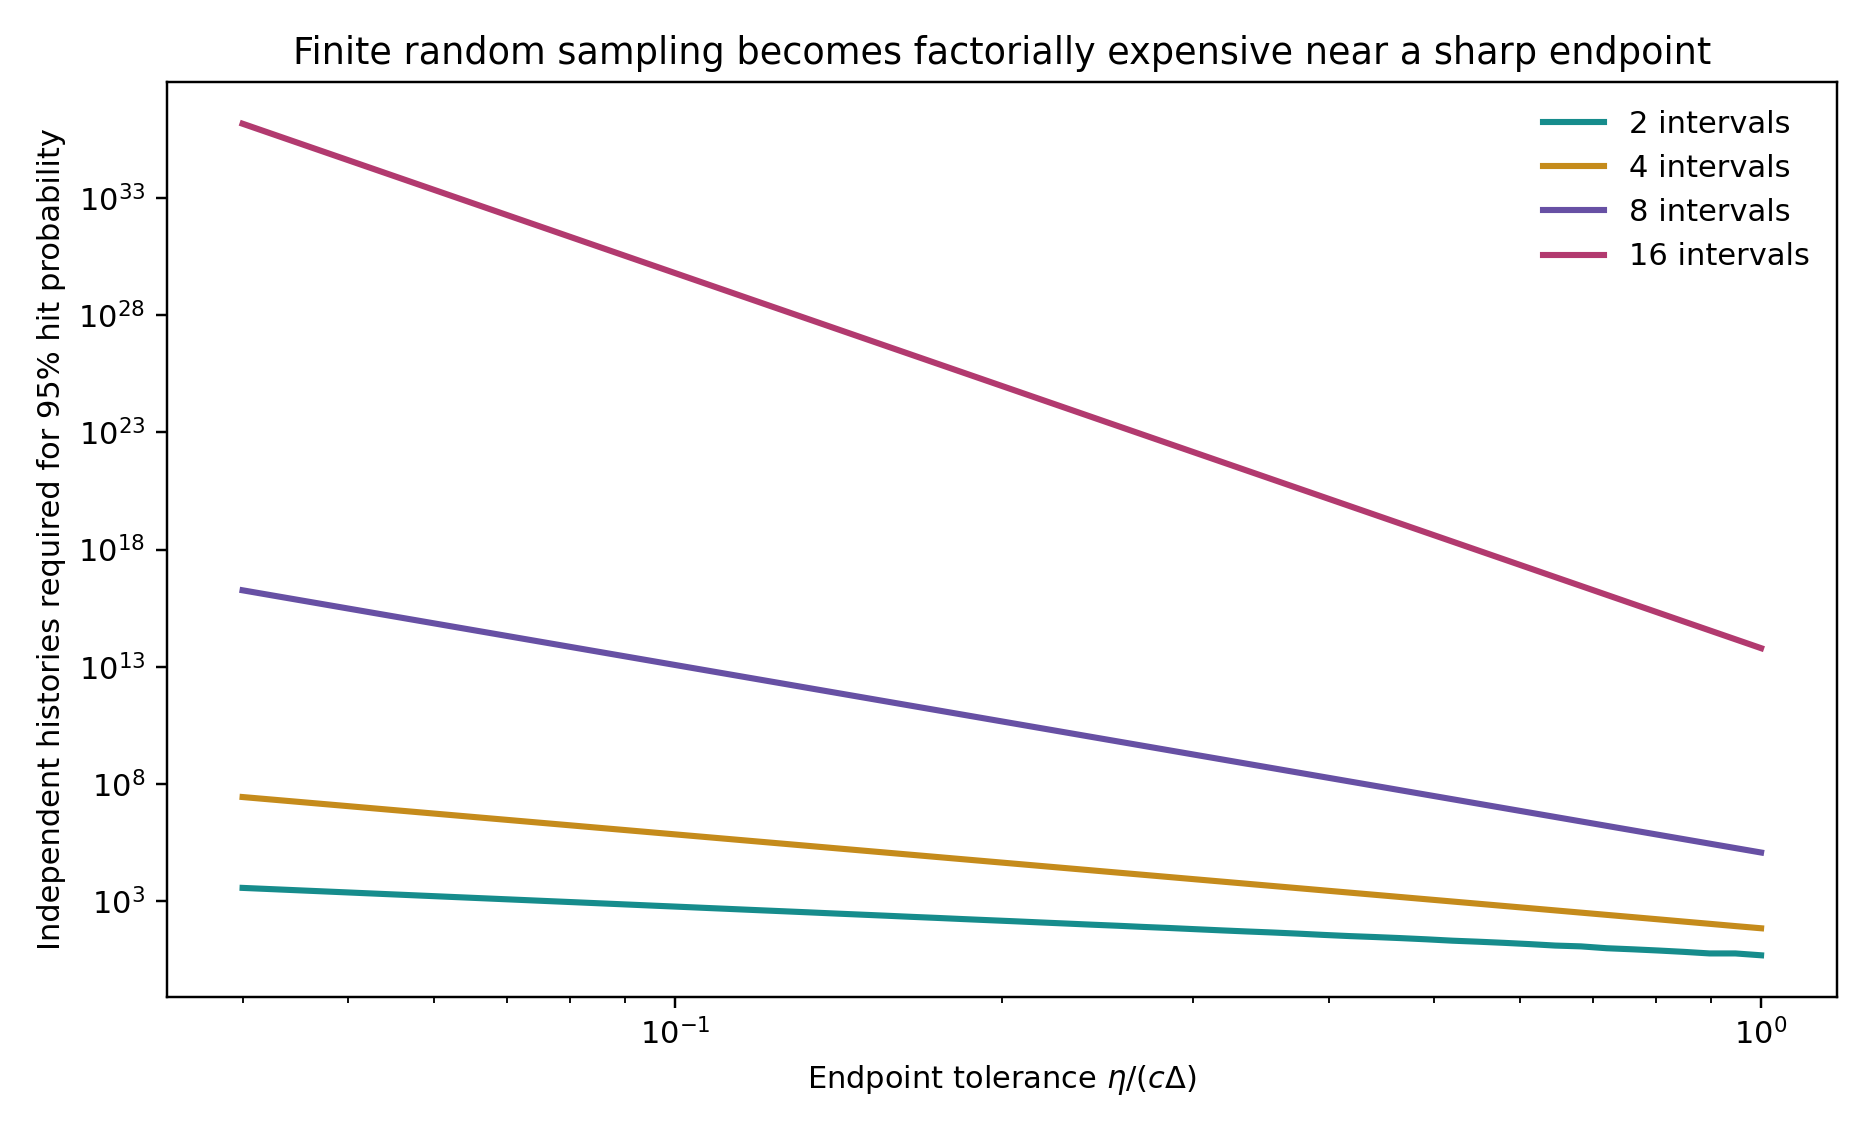
\includegraphics[width=0.88\linewidth]{figures/figure5_sampling_endpoint_cost.png}
\caption{Exact number of independent matched-sampler histories needed for a 95\% chance of approaching the maximal-loss endpoint. The cost grows factorially with the number of independently sampled intervals.}
\label{fig:samplingcost}
\end{figure}

\begin{figure}[t]
\centering
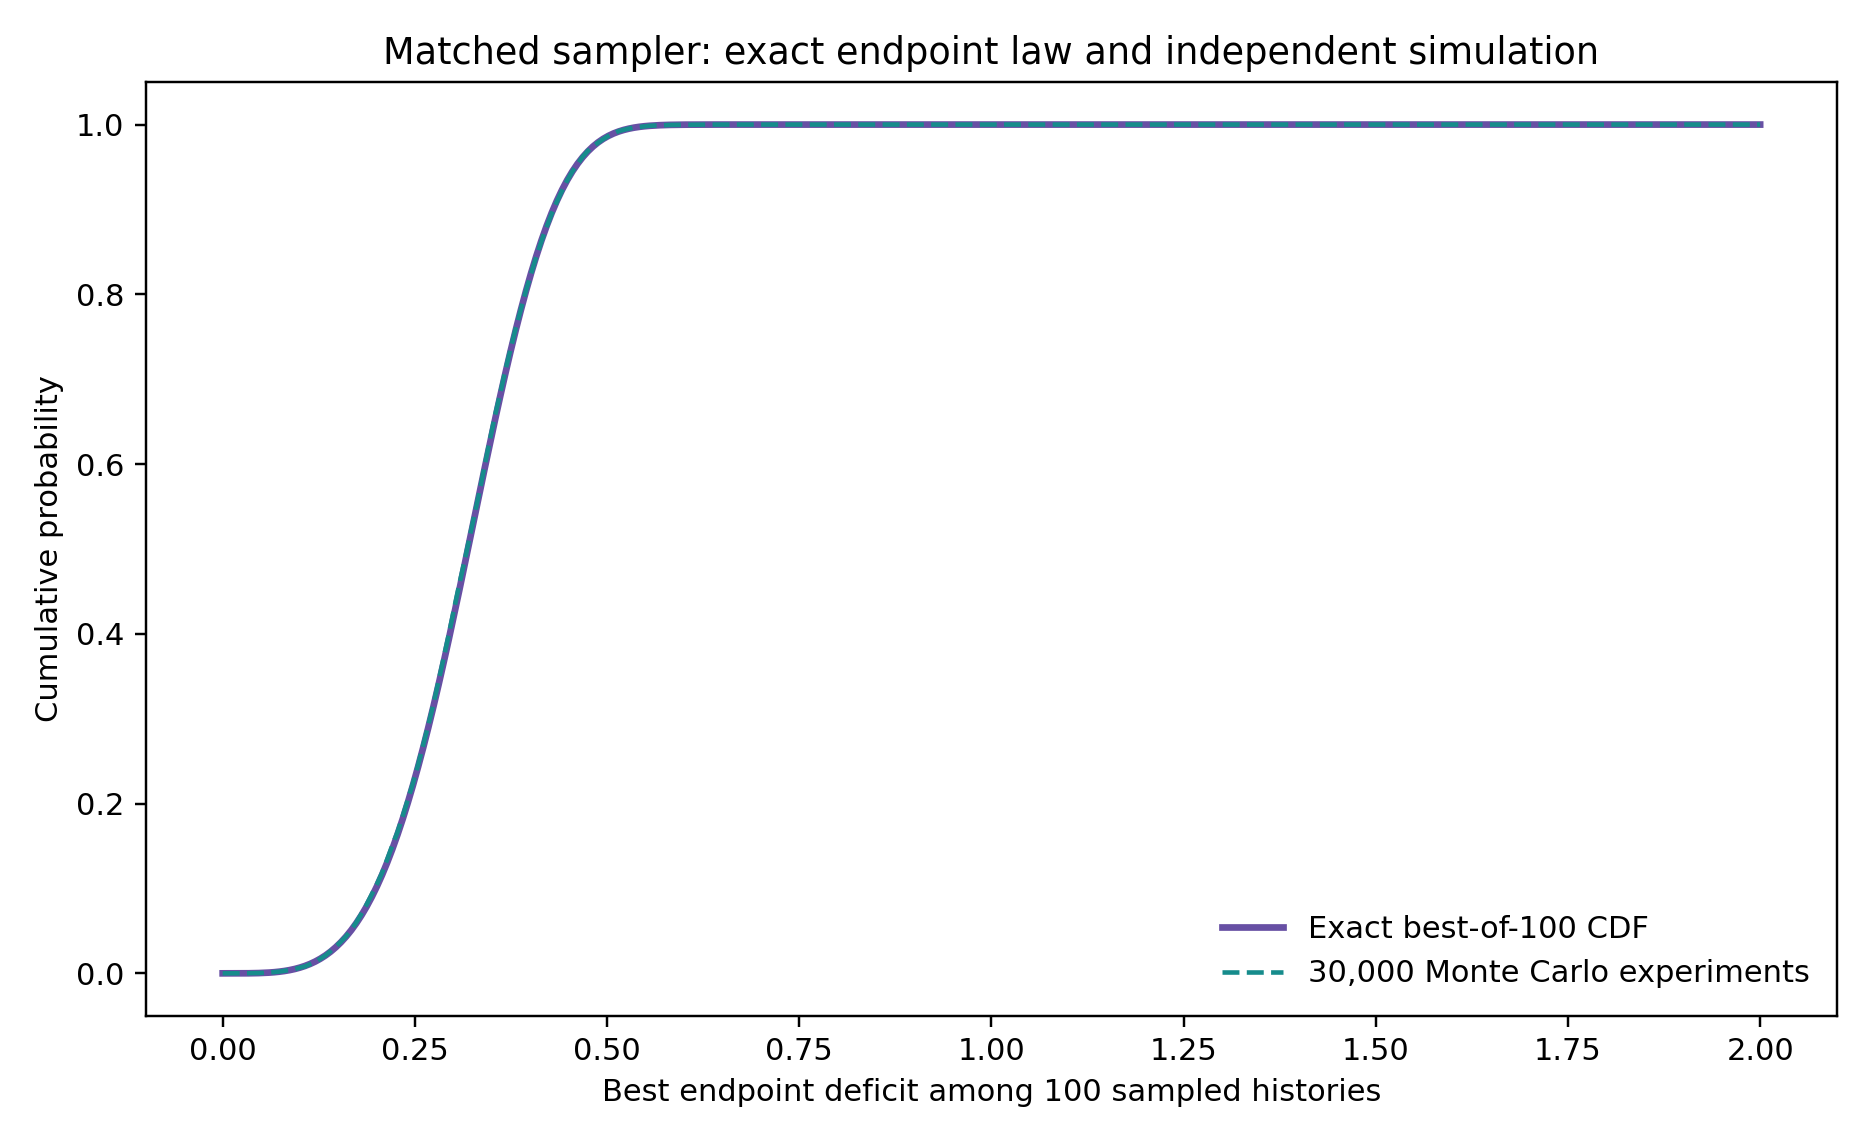
\includegraphics[width=0.88\linewidth]{figures/figure6_sampling_best_deficit.png}
\caption{Exact best-of-100 endpoint-deficit distribution for four independently sampled intervals, compared with 30,000 direct Monte Carlo experiments. This validates the order-statistic calculation; it is not a benchmark of the CRABS package.}
\label{fig:samplingcheck}
\end{figure}

\section{External deterministic constraints}
Let
\begin{equation}
 M(\tau)=\frac{M_0}{F(\tau)} \label{eq:M}
\end{equation}
be the model-defined pulled lineage trajectory anchored at $M_0$ at the analysis origin. Define the associated deterministic diversity trajectory
\begin{equation}
 N_{\mathrm{det}}(\tau)=\frac{M(\tau)}{u(\tau)}=\frac{M_0}{q(\tau)}. \label{eq:Ndet}
\end{equation}
This is a deterministic model quantity. It is not, without an observation model, the realised species richness of a historical clade.

A supplied model-scale statement $N_{\mathrm{det}}(\tau_i)\geq D_i$ is equivalent to
\begin{equation}
 q(\tau_i)\leq\frac{M_0}{D_i},\qquad
 n(x_i)\geq x_i-\frac{M_0}{D_i}. \label{eq:divconstraint}
\end{equation}

\begin{corollary}[Minimum cap implied by one deterministic diversity bound]\label{cor:diversity}
With no interior event between the analysis origin and $x_i>1$, the minimum cap compatible with \eqref{eq:divconstraint} is
\begin{equation}
 c_{\min}=\left[1-\frac{M_0/D_i-\rho}{x_i-1}\right]_+. \label{eq:diversitycap}
\end{equation}
For a shallower scale $x<x_i$, the same constraint implies
\begin{equation}
 n(x)\geq x_i-\frac{M_0}{D_i}-c(x_i-x), \label{eq:backprop}
\end{equation}
so information at an older age propagates towards the analysis origin.
\end{corollary}

The algebra is exact for $N_{\mathrm{det}}$. Applying it to fossil observations requires three further bridges: from the deterministic trajectory to a realised latent richness process, from preserved occurrences to latent richness, and from genera or higher taxa to the species scale. An incompatibility therefore falsifies the cap and those bridge assumptions jointly, not the cap alone.

\section{Plug-in mammal sensitivity illustration}
The public data and code of \textcite{upham2021} include pulled-rate estimates for mammal timetrees and fossil-genus summaries. We use one extracted trajectory only. The source tree was sliced at 1 Ma, so the analysis origin contains $M_0=4{,}790$ lineages; this is not present-day mammal diversity. The calculation holds $F$ fixed and supplies no coverage claim.

At actual age 58.5 Ma ($\tau=57.5$ after the shifted origin), the extracted values are
\begin{equation}
 \lambda_p=0.0438809486\ \mathrm{Myr}^{-1},\qquad F=119.7090495. \label{eq:mammalpoint}
\end{equation}
Under $c=0.5$ and no external deterministic constraint,
\[
 0.04388095\leq\lambda\leq0.08703484,
\]
a factor of 1.98343. Treating the cross-bin value $D=44$ as a purely illustrative lower bound changes the interval to
\[
 0.04825254\leq\lambda\leq0.08703484,
\]
a factor of 1.80374. Values $D=398$ and $D=577$ are incompatible with $c=0.5$ under the full deterministic and taxonomic mapping; their minimum compatible caps are 0.90704 and 0.93849. These numbers diagnose assumptions. They do not estimate mammalian turnover or validate a genus-to-species bridge.

\begin{figure}[t]
\centering
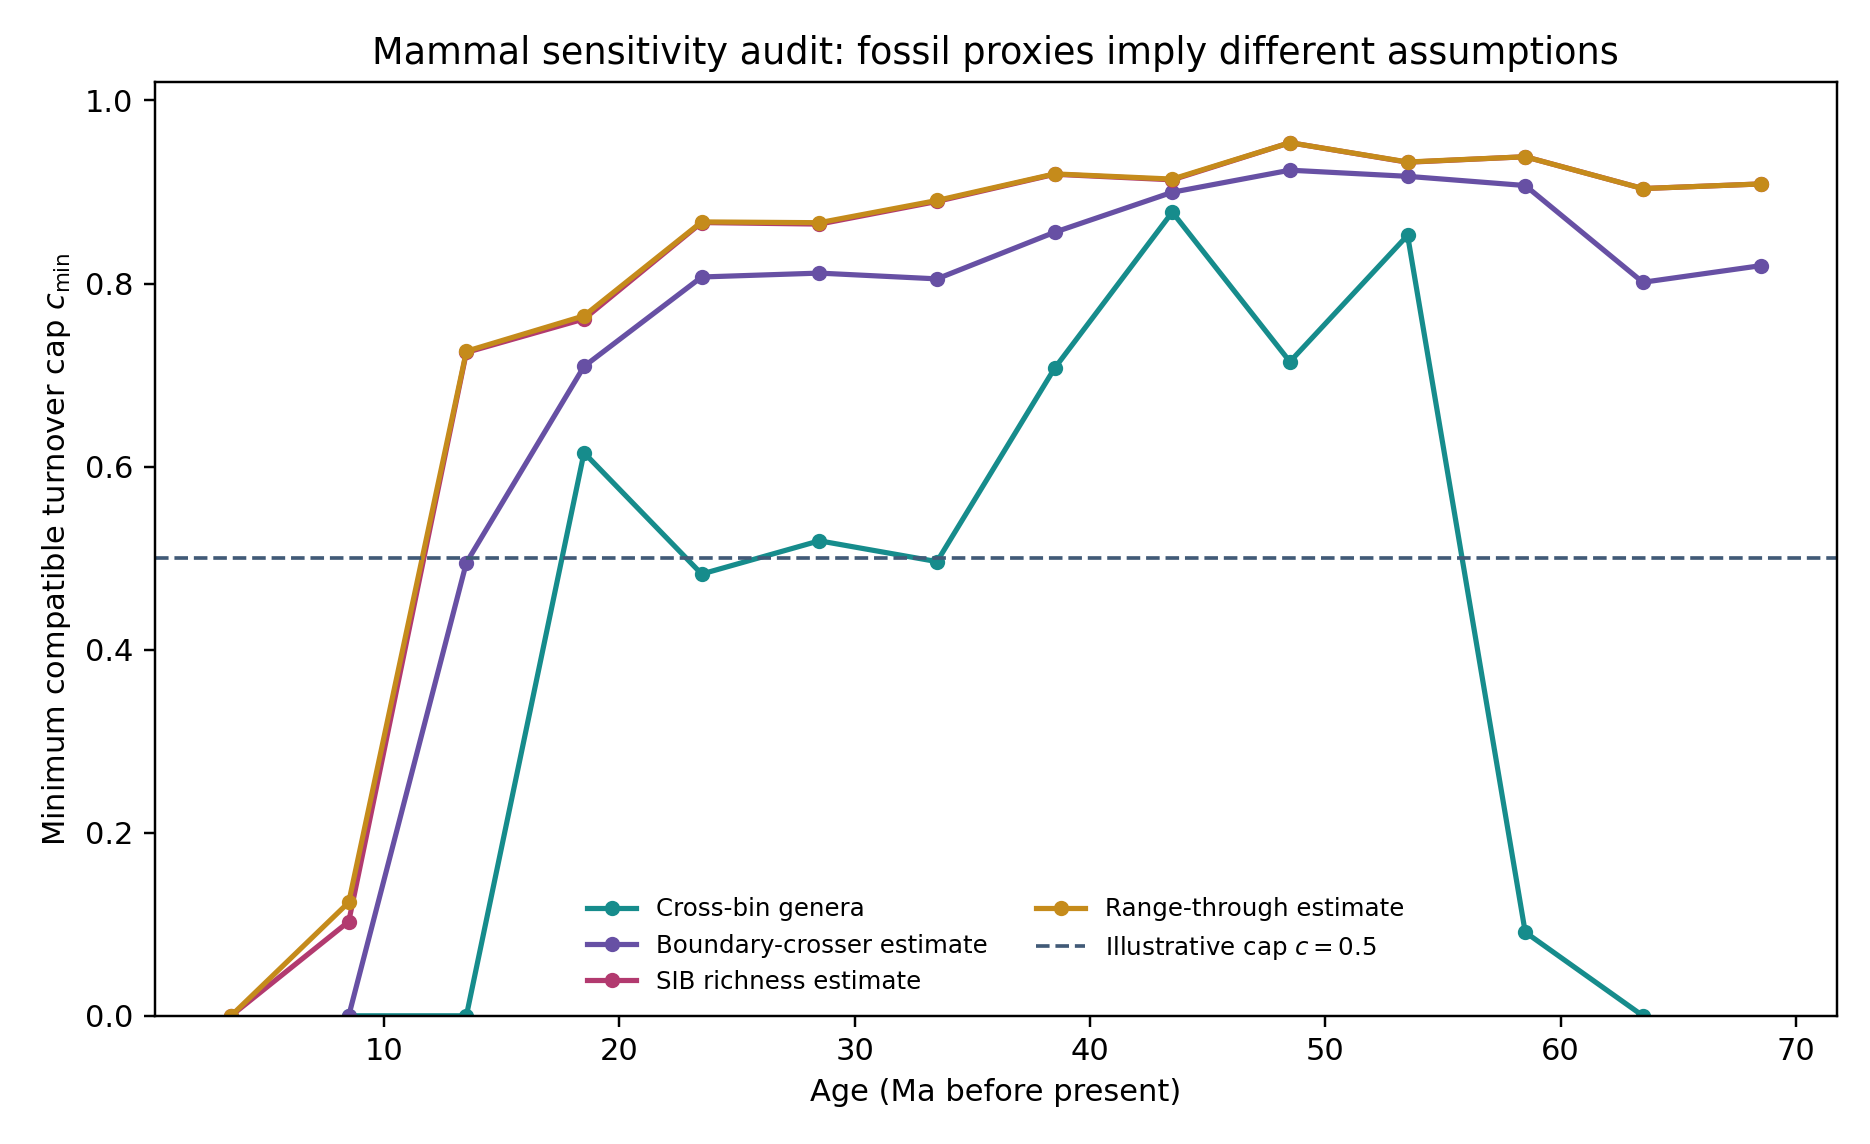
\includegraphics[width=0.88\linewidth]{figures/figure2_mammalia_turnover_audit.png}
\caption{Single-tree plug-in sensitivity with no simultaneous signal band or fossil observation model. Different fossil-genus summaries imply different minimum caps only under the stated deterministic and taxonomic mappings.}
\label{fig:mammalaudit}
\end{figure}

\begin{figure}[t]
\centering
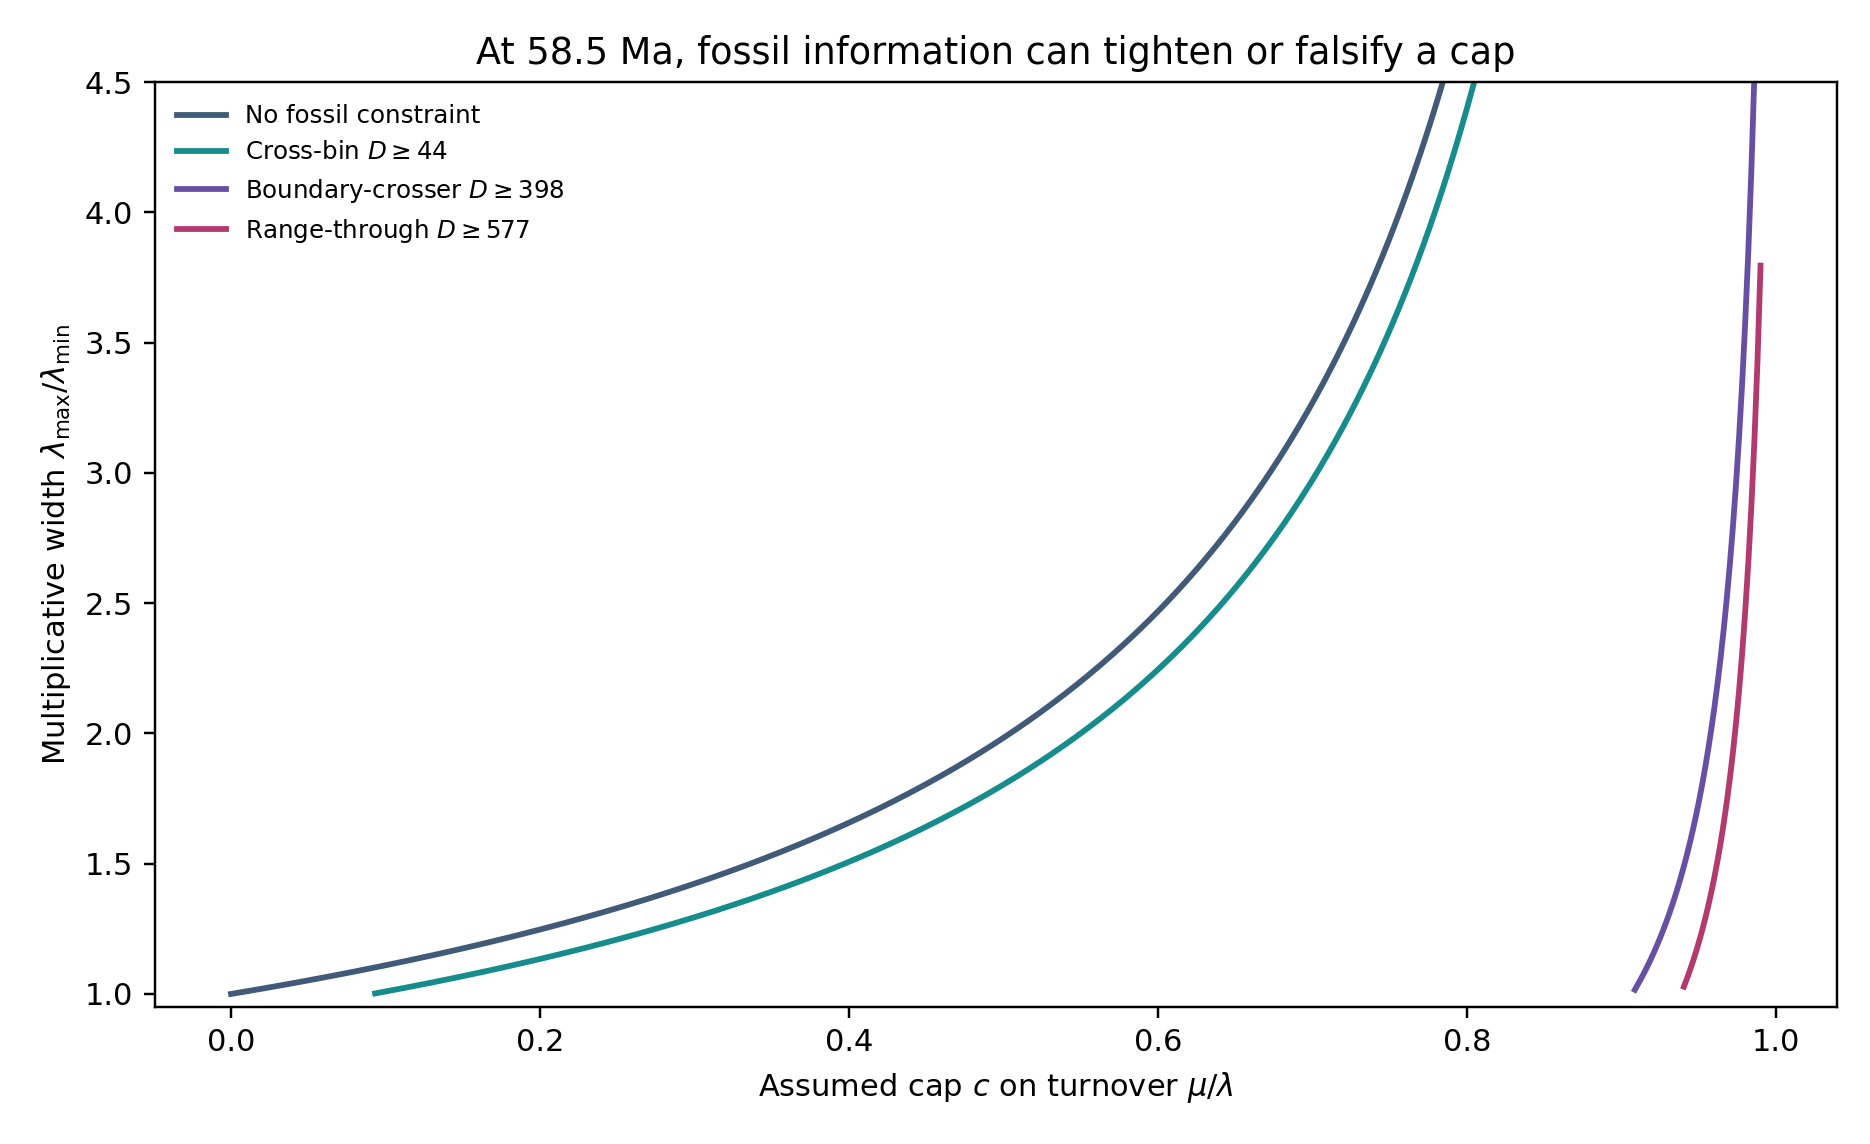
\includegraphics[width=0.88\linewidth]{figures/figure3_worked_sensitivity.png}
\caption{Worked plug-in sensitivity at 58.5 Ma. Curves report conditional mathematical compatibility, not confidence intervals or realised palaeodiversity.}
\label{fig:mammalworked}
\end{figure}

\begin{figure}[t]
\centering
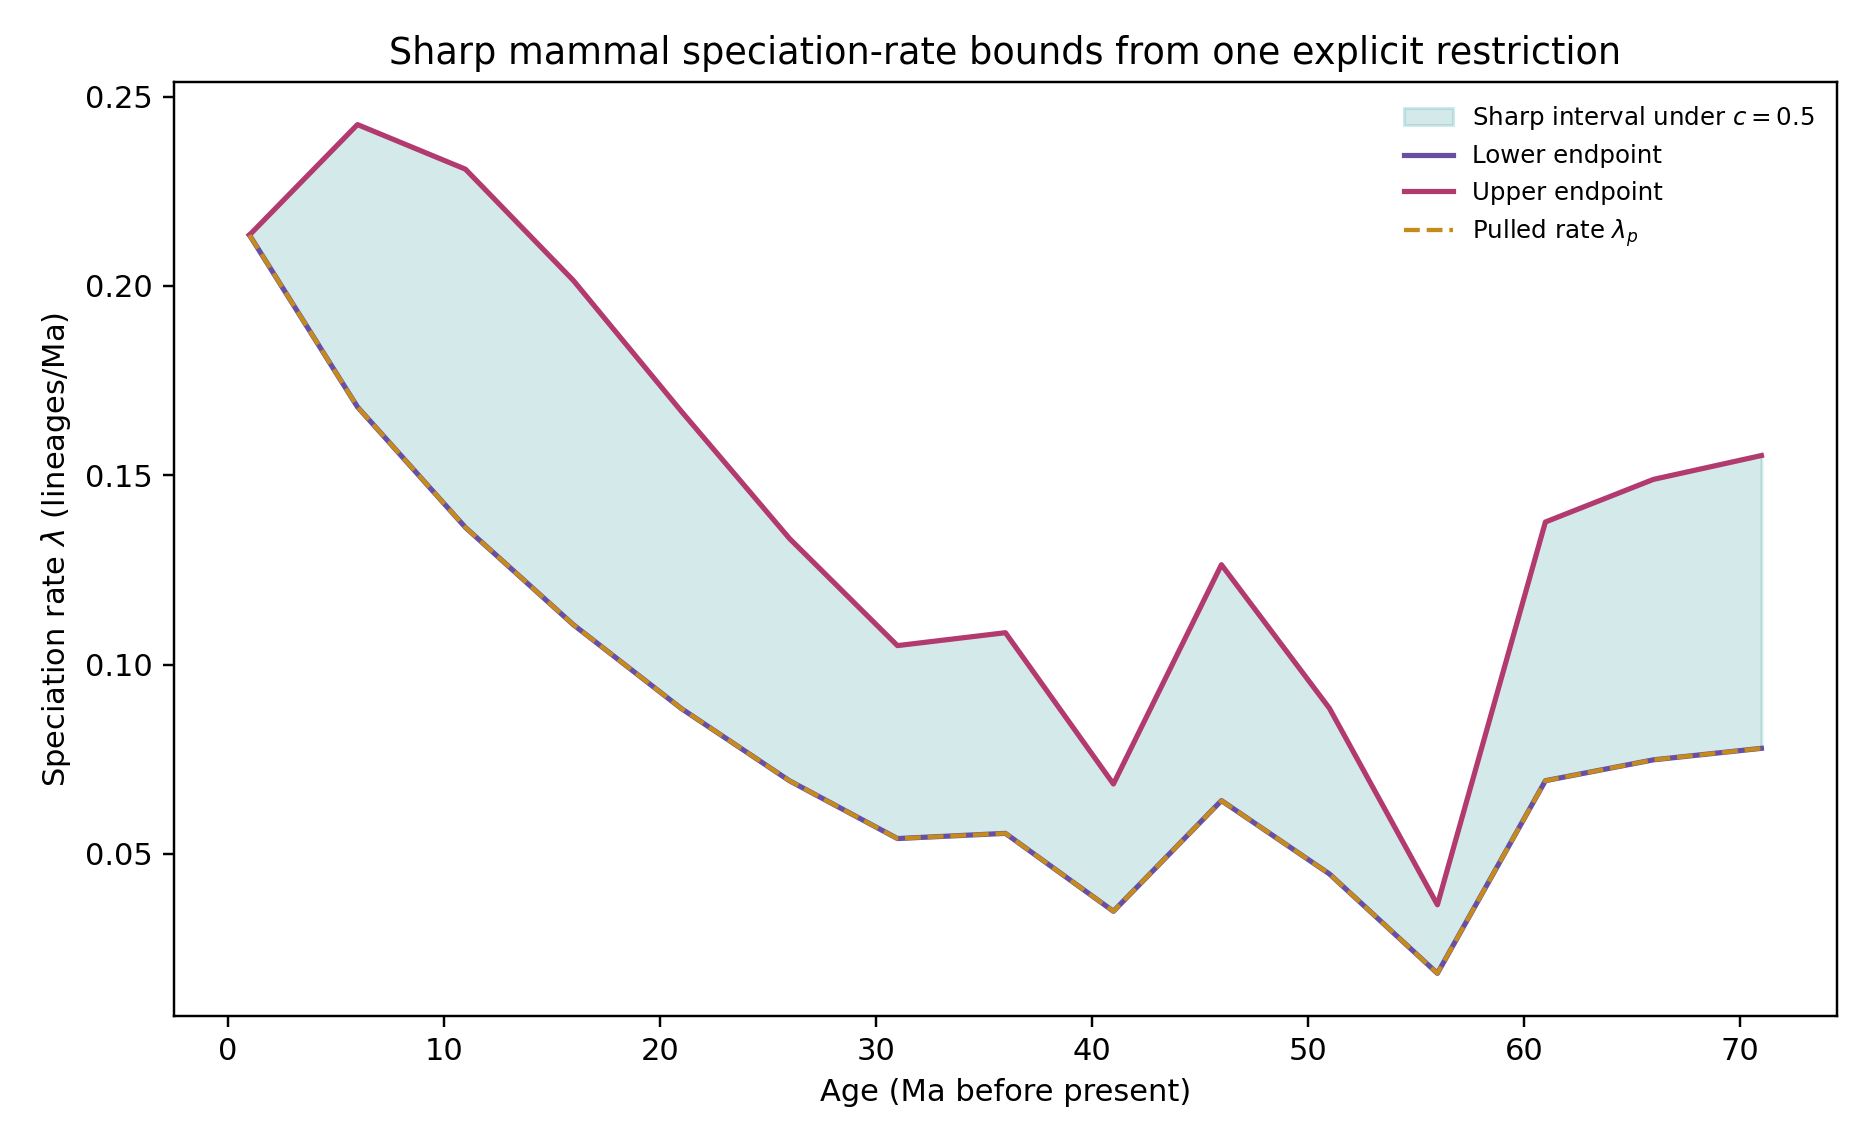
\includegraphics[width=0.88\linewidth]{figures/figure4_mammalia_lambda_bounds.png}
\caption{Sharp pointwise speciation bounds under $c=0.5$ for one fixed mammal pulled-rate curve. The restriction excludes continuous negative net diversification; the figure contains no pulled-signal uncertainty.}
\label{fig:mammalbounds}
\end{figure}

\section{Conditional geometry versus statistical uncertainty}
Let $\Theta(F)$ denote the conditional functional identified set generated by a pulled-scale trajectory $F$. Suppose a simultaneous random set $\Fset_{1-\alpha}$ satisfies
\begin{equation}
 \Pr(F_0\in\Fset_{1-\alpha})\geq1-\alpha. \label{eq:Fcoverage}
\end{equation}
Then
\begin{equation}
 \Theta(F_0)\subseteq\bigcup_{F\in\Fset_{1-\alpha}}\Theta(F)
 \quad\text{whenever }F_0\in\Fset_{1-\alpha}, \label{eq:coverageunion}
\end{equation}
so the union transfers the simultaneous coverage of the signal set to a set containing the true conditional identified set. This is a set-inclusion principle, not an operational inferential method. A pointwise band is not automatically simultaneous; this release does not construct $\Fset_{1-\alpha}$ or propagate phylogenetic, smoothing and model uncertainty.

\section{Position relative to existing methods}
\begin{table}[H]
\centering
\scriptsize
\renewcommand{\arraystretch}{1.08}
\begin{tabularx}{\linewidth}{@{}>{\raggedright\arraybackslash}p{0.19\linewidth}>{\raggedright\arraybackslash}X>{\raggedright\arraybackslash}X>{\raggedright\arraybackslash}X>{\raggedright\arraybackslash}X@{}}
\toprule
Question & Louca--Pennell & Congruence exploration & Identifiable restricted or enriched models & Present candidate \\
\midrule
What is learned? & Pulled signal and congruence & Constructed or sampled histories; shared patterns & Point identification within stronger model or data classes & Conditional functional set and target projections \\
Endpoint guarantee & No & Proposal-dependent finite exploration & Point estimate under model & Closed-form sharp endpoints for stated classes \\
Infeasibility witness & No & Not the principal output & Model fit or identification result & Violating pair and minimum cap \\
Deterministic events & Process literature required & Event scenarios may be constructed & Model-specific & Stieltjes coordinate and fixed-stem proof \\
Pulled-signal uncertainty & Estimation problem remains & Method-specific & Method-specific & Not supplied; union architecture only \\
\bottomrule
\end{tabularx}
\caption{The proposed method complements rather than supersedes existing approaches. Congruence tools explore histories; identifiable restrictions or richer observations can restore point identification \parencite{legried2022,legried2023,truman2025,truman2026correction,dieselhorst2026}.}
\label{tab:comparison}
\end{table}

The integrating factor, pulled scale and zero-inflated geometric branching laws have reconstructed-process antecedents \parencite{lambert2013,hohna2015,macpherson2022}. Partial-identification framing, generic Lipschitz extensions and infinite-dimensional linear programming are also established literatures \parencite{manski2003,mcshane1934,whitney1934,anderson1987}. The defensible priority claim is narrower: we found no prior work coupling this cumulative-loss measure fibre to the complete package of cap-regime bounds, finite certificates, barrier test, minimum-cap diagnostic and exact endpoint-sampling law. The search was targeted, not systematic. A specialist recognition check remains necessary.

\section{Computational assurance}
Release 0.2.1 includes:
\begin{itemize}
\item 17 deterministic unit tests covering the smooth chart, cap regimes, event algebra, fixed-stem normalisation, finite certificates, boundary validation, mammal replay and sampling theorem;
\item an independently written loop-based envelope implementation and 720 linear-programme endpoint checks across 180 random feasible cases;
\item a direct 160,000-replicate birth--death simulation with two deterministic bottlenecks, checked against analytic survival and the conditional descendant-count law;
\item five deliberately broken or infeasible negative controls, all detected;
\item exact dependency records, component-level licences, claim-to-evidence mappings and scoped assurance states;
\item machine-readable data and alt text for every figure, plus PDF render inspection.
\end{itemize}
These checks establish internal replay and independent numerical consistency. They do not constitute external mathematical review, biological validation or formal proof checking. Exact dependencies are recorded, and the complete check suite passes under normal and optimized Python in a clean container pinned to a Python 3.13.5 base-image digest. That recreation was performed by the release-preparing agent, so independent external reproduction remains unassessed.

\section{Limitations and research programme}
The release remains a candidate for five reasons. First, the fixed-stem theorem needs an external specialist audit and does not cover crown or random-origin conditioning. Second, statistical inference requires a simultaneous uncertainty set for the pulled signal. Third, fossil application requires a preservation, observation and taxonomic mapping model. Fourth, the matched sampling theorem should be complemented by an actual CRABS comparison under identical restrictions. Fifth, priority should be checked across stochastic-process, survival-analysis, viability, optimal-recovery and non-English literatures.

The most valuable extensions are: exact robust envelopes over a simultaneous family of $F$ curves; observation-aware fossil inequalities or chance constraints; target-specific optimisation for peak timing and integrated extinction; crown-conditioned event laws; and formalisation of Theorems 1, 6 and 8 in a proof assistant.

\section{Conclusion}
A congruence class is a functional identified set, not a collection of curves returned by one sampler. The cumulative-loss coordinate makes a useful part of that set affine. Under explicit restrictions, the analyst can report feasible trajectories, exact target endpoints, endpoint-attaining histories and short incompatibility certificates. The cap extension also identifies the boundary at which continuous decline destroys finite upper identification. These results provide a mathematically exact complement to exploration and point-identifying models. Their empirical use must retain the same discipline: fixed-signal geometry, statistical uncertainty and biological observation models are separate layers.

\appendix
\section{Sanity checks}
\paragraph{Complete-sampling pure birth.}
With $\nu=0$, $A=0$, $u=1$, $q=F$, $\lambda=\lambda_p$ and $\mu=0$. With incomplete sampling but no extinction, $\nu=(1-\rho)\delta_0$.

\paragraph{Constant turnover.}
If $\rho=1$ and $\dd\nu=c\dd F$, then
\[
 A=c(F-1),\qquad q=1+(1-c)(F-1),\qquad
 \lambda=\frac{\lambda_pF}{1+(1-c)(F-1)},
\]
and $\dd\nu/\dd F=c=\mu/\lambda$.

\paragraph{Instantaneous event.}
For $m=(1-s)q(a-)$,
\[
 \frac{u(a+)}{u(a-)}=\frac{q(a+)}{q(a-)}=s
\]
exactly.

\paragraph{Fixed-stem normalisation.}
For $n$ sampled descendants, integrating \eqref{eq:unconditionedtree} over the ordered simplex gives
\[
 \frac{u(T)}{F(T)}\left(1-\frac1{F(T)}\right)^{n-1}=p_n(T),
\]
which checks both the topology-marginal branching-time multiplicity factor and the event-invariant $p_1/u$ ratio.

\paragraph{Endpoint sampling.}
For $m=1$, \eqref{eq:smalltail} reduces to the uniform distribution on $[0,c\Delta]$. For $m=2$, it gives the triangular lower tail $\eta^2/[2(c\Delta)^2]$.

\section{Reproduction commands}
From the release root:
\begin{verbatim}
make verify
make verify-package
docker build -f Containerfile -t affine-diversification-fibres:0.2.1 .
docker run --rm affine-diversification-fibres:0.2.1
\end{verbatim}

\printbibliography
\end{document}
